%%%%%%%%%%%%%%%%%%%%%%%%%%%%%%%%%%%%%%
% LaTeX style based off of:
% http://www.nathanieljohnston.com/2009/08/latex-poster-template/
% By Nathaniel Johnston
%%%%%%%%%%%%%%%%%%%%%%%%%%%%%%%%%%%%%%

\documentclass[final]{beamer}
\usepackage[scale=1.24]{beamerposter}
\usepackage{graphicx}			% allows us to import images

%-----------------------------------------------------------
% Custom commands that I use frequently
%-----------------------------------------------------------

\newcommand{\bb}[1]{\mathbb{#1}}
\newcommand{\cl}[1]{\mathcal{#1}}
\newcommand{\fA}{\mathfrak{A}}
\newcommand{\fB}{\mathfrak{B}}
\newcommand{\Tr}{{\rm Tr}}
\newtheorem{thm}{Theorem}

%-----------------------------------------------------------
% Define the column width and poster size
% To set effective sepwid, onecolwid and twocolwid values, first choose how many columns you want and how much separation you want between columns
% The separation I chose is 0.024 and I want 4 columns
% Then set onecolwid to be (1-(4+1)*0.024)/4 = 0.22
% Set twocolwid to be 2*onecolwid + sepwid = 0.464
%-----------------------------------------------------------

\newlength{\sepwid}
\newlength{\onecolwid}
\newlength{\twocolwid}
\setlength{\paperwidth}{48in}
\setlength{\paperheight}{36in}
\setlength{\sepwid}{0.024\paperwidth}
\setlength{\onecolwid}{0.22\paperwidth}
\setlength{\twocolwid}{0.464\paperwidth}
\setlength{\topmargin}{-0.5in}
\usetheme{confposter}
\usepackage{exscale}

\usepackage{booktabs}
%-----------------------------------------------------------
% The next part fixes a problem with figure numbering. Thanks Nishan!
% When including a figure in your poster, be sure that the commands are typed in the following order:
% \begin{figure}
% \includegraphics[...]{...}
% \caption{...}
% \end{figure}
% That is, put the \caption after the \includegraphics
%-----------------------------------------------------------

\usecaptiontemplate{
\small
\structure{\insertcaptionname~\insertcaptionnumber:}
\insertcaption}

%-----------------------------------------------------------
% Define colours (see beamerthemeconfposter.sty to change these colour definitions)
%-----------------------------------------------------------

%\setbeamercolor{block title}{fg=ngreen,bg=white}
%\setbeamercolor{block body}{fg=black,bg=white}
%\setbeamercolor{block alerted title}{fg=white,bg=dblue!70}
%\setbeamercolor{block alerted body}{fg=black,bg=dblue!10}

\setbeamercolor{block title}{fg=HarvardCrimson,bg=white}
\setbeamercolor{block body}{fg=black,bg=white}
\setbeamercolor{block alerted title}{fg=white,bg=dblue!70}
\setbeamercolor{block alerted body}{fg=black,bg=dblue!10}


%-----------------------------------------------------------
% Name and authors of poster/paper/research
%-----------------------------------------------------------
\newcommand{\footleft}{\textit{The 11th Workshop on Innovative Use of NLP for Building Educational Applications, AESW 2016 Shared Task}}
\newcommand{\footright}{\{schmaltz@fas,yoonkim@seas,srush@seas,shieber@seas\}.harvard.edu}
\title{Sentence-Level Grammatical Error Identification
\vskip0.4ex \\as Sequence-to-Sequence Correction}
\author{Allen Schmaltz \and Yoon Kim \and Alexander M. Rush \and Stuart M. Shieber}
\institute{Harvard University, Cambridge, MA}

%-----------------------------------------------------------
% Start the poster itself
%-----------------------------------------------------------
% The \rmfamily command is used frequently throughout the poster to force a serif font to be used for the body text
%-----------------------------------------------------------

\begin{document}
\begin{frame}[t]
  \begin{columns}[t]												% the [t] option aligns the column's content at the top
%%%%%%%%%%%%%%%%%%%%%%%%%%%%%%%%%%%%%%
% The left (i.e., 0) column
%%%%%%%%%%%%%%%%%%%%%%%%%%%%%%%%%%%%%%     
    \begin{column}{\sepwid}\end{column}			% empty spacer column
    \begin{column}{\onecolwid}
%%%%%%%%%%%%%%%%%%%
      \begin{alertblock}{The Binary Classification Task}
        \rmfamily{The Automated Evaluation of Scientific Writing (AESW) \textbf{Shared Task} 2016: Given a sentence, determine whether it needs to be edited (i.e., contains a grammatical error, broadly construed).}
      \end{alertblock}
%%%%%%%%%%%%%%%%%%%
      \vskip2ex
%%%%%%%%%%%%%%%%%%%
      \begin{block}{Data}
        \rmfamily{
        \begin{itemize}
            \item The AESW dataset is the first large-scale, publicly available professionally edited dataset of academic, scientific writing
            \item A collection of nearly 10,000 scientific journal articles (Engineering, Computer Science, Mathematics, Chemistry, Physics, etc.)
            \item Training set consists of about 500,000 sentences with errors and an additional 700,000 that are error-free
            \item Errors are described at the token level with insert and delete tags (see diagram at right)
            \end{itemize}}
      \end{block}
%%%%%%%%%%%%%%%%%%%      
      \vskip2ex
%%%%%%%%%%%%%%%%%%%
      \begin{block}{Approach}
        \rmfamily{
        \begin{itemize}
        	\item To establish a strong baseline on this new dataset, we utilize a CNN for binary classification, experimenting with word2vec:
        	\vskip0.5ex
			\begin{itemize}
				\item Keeping the word vectors static (\textsc{CNN-static}) 
				\item Fine-tuning the vectors (\textsc{CNN-nonstatic})
			\end{itemize}
			\vskip0.5ex
        	\item We propose two encoder-decoder architectures for this task, recasting the problem as translation (incorrect $\rightarrow$ correct) in order to train at the lowest granularity of annotations: 
        	\vskip0.5ex
			\begin{itemize}
				\item A word-based model (\textsc{Word})
				\item A character-based model (\textsc{Char})
			\end{itemize}
			\vskip0.5ex
        %\item For the encoder-decoder models, beam search is used to identify the highest scoring sentence
		\item Evaluation is via $F_1$ at the sentence level
		\item On the final run on test, we use an ensemble of multiple encoder-decoder models and a CNN classifier (\textsc{Combination})
        \end{itemize}}
      \end{block}
%%%%%%%%%%%%%%%%%%%
        \vskip2ex
        \begin{block}{Acknowledgements}
          \small{\rmfamily{We would like to thank the Institute for Quantitative Social Science (IQSS) and the Harvard Initiative for Learning and Teaching (HILT) for support and Jeffrey Ling for software development.}} \\
        \end{block}
    \end{column}

%%%%%%%%%%%%%%%%%%%%%%%%%%%%%%%%%%%%%% 
% Second from left column--i.e., column 1 (Note that columns 1 and 2 are merged for the architecture image)
%%%%%%%%%%%%%%%%%%%%%%%%%%%%%%%%%%%%%% 
    \begin{column}{\sepwid}\end{column}			% empty spacer column
    \begin{column}{\twocolwid}							% create a two-column-wide column and then we will split it up later
      \begin{columns}[t,totalwidth=\twocolwid]	% split up that two-column-wide column
        \begin{column}{\onecolwid}\vspace{-.69in}
%%%%%%%%%%%%%%%%%%%
            \begin{block}{Encoder-Decoder vs. CNN}
                \begin{table}[ht!]
                    \centering
                    \small
                    \begin{tabular}{lcccc}
                    \toprule
                    Model & Data & Precision & Recall & $F_1$ \\
                    \midrule
                    \textsc{Random} & N/A & $0.3885$ & $0.4992$ & $0.4369$ \\
                    \midrule
                    \textsc{CNN-static} & Training+word2vec & $0.5349$ & $0.7586$ & $0.6274$ \\
                    \textsc{CNN-nonstatic} & Training+word2vec & $0.5365$ & $0.7758$ & $0.6343$ \\
                    \midrule
                    \textsc{Word+all} & Training & $0.5399$ & $0.7882$ & $0.6408$ \\
                    \textsc{Word+sample} & Training & $0.5394$ & $0.8024$ & $0.6451$ \\
                    \textsc{Char+all} & Training & $0.5400$ & $0.8048$ & $0.6463$ \\
                    \textsc{Char+sample} & Training & $0.5526$ & $0.8126$ & $0.6579$ \\
                    \bottomrule
                    \end{tabular}
                    \caption{\rmfamily{Experimental results on the development set excluding the held-out 10k tuning subset.}}
                    \label{tab:dev-results}
                \end{table}
                \begin{itemize}
                    \item The encoder-decoder models (and \textsc{Char} in particular) improve over the CNN models, at the expense of training/testing time.
                    \item The \textsc{+sample} models are given a random sample of 200,000 sentences without edits and perform better than those given all error-free sentences (\textsc{+all}). See also Figure 1.
                \end{itemize}
            \end{block}
%%%%%%%%%%%%%%%%%%%
        \end{column}
%%%%%%%%%%%%%%%%%%%%%%%%%%%%%%%%%%%%%%
% Column index 2 (second from right)
%%%%%%%%%%%%%%%%%%%%%%%%%%%%%%%%%%%%%%
        \begin{column}{\onecolwid}\vspace{-.69in}
        \setbeamercolor{block alerted title}{fg=black,bg=StanfordPantone5665} % Change the alert block title colors
        \setbeamercolor{block alerted body}{fg=black,bg=white} % Change the alert block body colors

%%%%%%%%%%%%%%%%%%%
            \begin{alertblock}{Contributions}
                \rmfamily{
                    \begin{itemize}
                        \item Highest performing system (ensemble, as well as \textsc{Char} separately) on the binary classification Shared Task
                        \item Demonstrated utility of a neural attention-based model for sentence-level grammatical error identification 
                        \item Our end-to-end approach does not have separate components for candidate generation or re-ranking that make use of hand-tuned rules or explicit syntax, nor do we employ separate classifiers for human-differentiated subsets of errors 
                        \item Evidence to suggest modeling at the sub-word level is beneficial
                    \end{itemize}
                }
            \end{alertblock}
%%%%%%%%%%%%%%%%%%% 
        \end{column}
%%%%%%%%%%%%%%%%%%%%%%%%%%%%%%%%%%%%%%
        \end{columns}
%%%%%%%%%%%%%%%%%%%%%%%%%%%%%%%%%%%%%%
% The two center columns are merged for the image below
%%%%%%%%%%%%%%%%%%%%%%%%%%%%%%%%%%%%%%
        %\vskip2.5ex
        \centering
        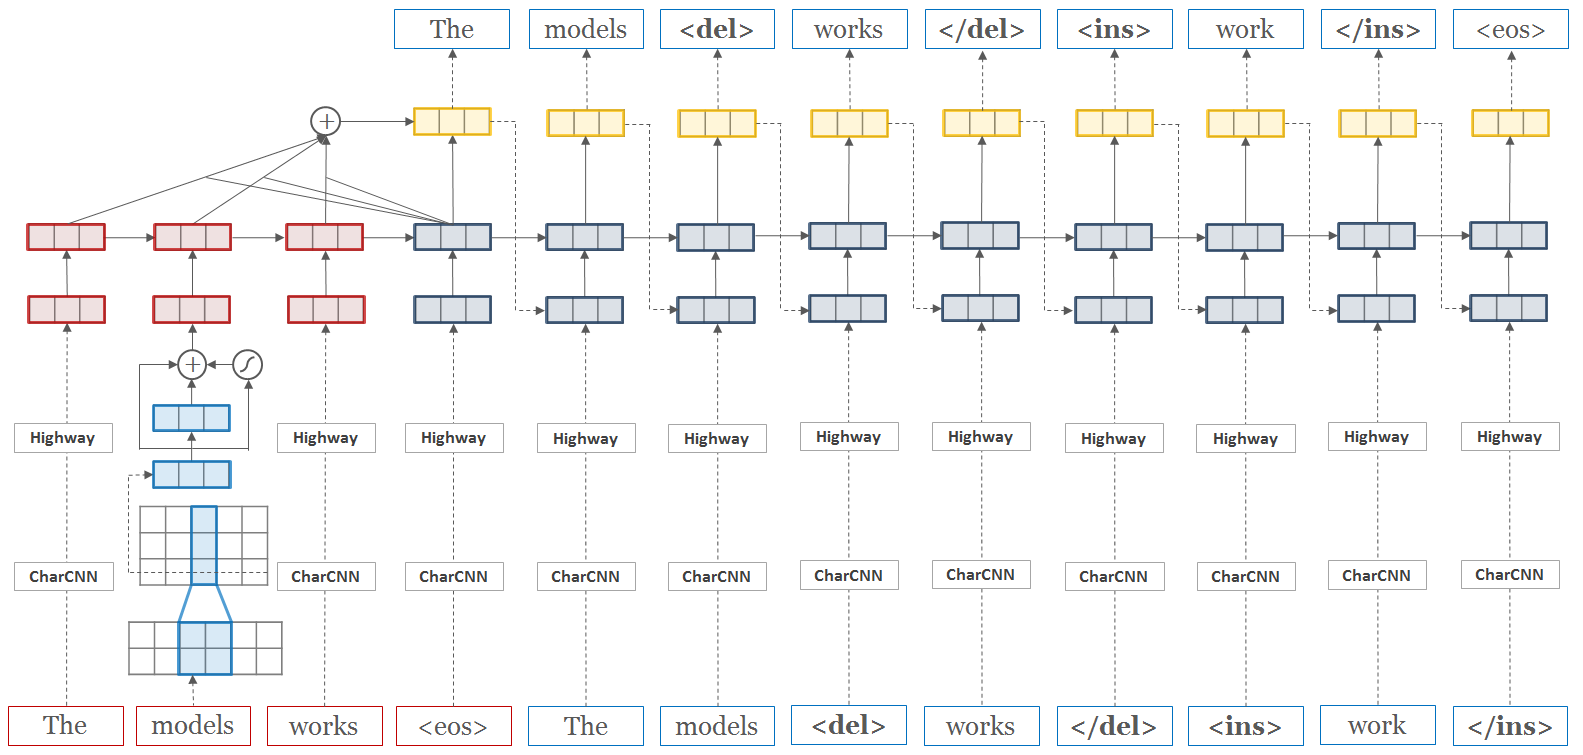
\includegraphics[width=.9\columnwidth]{figures/grammar}
        \vskip1.0ex
            \begin{alertblock}{Character-aware Encoder-Decoder Architecture (\textsc{Char})}		% an ACTUAL two-column-wide column
                \rmfamily{ Illustration (above) of the \textsc{Char} model architecture translating an example source sentence into the corrected target 
                \begin{itemize} \small
                    \item A CNN is applied over character embeddings to obtain a fixed dimensional representation of a word, which is given to a highway network (in light blue, above). 
                    \item Output from the highway network is used as input to a LSTM encoder-decoder. 
                    \item At each step of the decoder, its hidden state is interacted with the hidden states of the encoder to produce attention weights (for each word in the encoder), which are
                                    used to obtain the context vector via a convex combination. 
                    \item The context vector is combined with the decoder hidden state through a one layer MLP (yellow), after which an affine 
                                    transformation followed by a softmax is applied to obtain a distribution over the next word/tag.
                    \item The MLP layer (yellow) is used as additional input (via concatenation) for the next time step.
                    \item An equality check between the source and the highest scoring output sentence (via beam search) determines the binary label.
                    %\item Generation continues until the $<$\texttt{eos}$>$ symbol is generated.
                \end{itemize}}
            \end{alertblock}
        \end{column}
  
%ORIGINAL CAPTION FROM THE PAPER: \caption{\footnotesize An illustration of the \textsc{Char} model architecture translating an example source sentence into the corrected target with a single word replacement. A CNN (here, with three filters of width two) is applied over character embeddings to obtain a fixed dimensional representation of a word, which is given to a highway network (in light blue, above). Output from the highway network is used as input to a LSTM encoder/decoder. At each step of the decoder, its hidden state is interacted with the hidden states of the encoder to produce attention weights (for each word in the encoder), which are
%used to obtain the context vector via a convex combination. The context vector is combined 
%with the decoder hidden state through a one layer MLP (yellow), after which an affine 
%transformation followed by a softmax is applied to obtain a distribution over the next word/tag.
%The MLP layer (yellow) is used as additional input (via concatenation) for the next time step.
%Generation continues until the $<$\texttt{eos}$>$ symbol is generated.}
%%%%%%%%%%%%%%%%%%%%%%%%%%%%%%%%%%%%%%
% Column 3 (right-most)
%%%%%%%%%%%%%%%%%%%%%%%%%%%%%%%%%%%%%%
  \begin{column}{\sepwid}\end{column}			% empty spacer column
  \begin{column}{\onecolwid}
%%%%%%%%%%%%%%%%%%%
      \begin{block}{Tuning}
       	\begin{itemize}
			\item Post-hoc tuning was necessary to avoid under-prediction
			\begin{itemize}
				\item \textbf{CNN models}: tuned the decision boundary to maximize the $F_1$-score on the held-out tuning set
				\item \textbf{Encoder-decoder models}: tuned the bias weights (given as input to the final softmax layer generating the words/tags distribution) associated with the four annotation tags via a coarse grid search by iteratively running beam search on the tuning set
			\end{itemize}
       	\end{itemize}
        \begin{figure}[htb]
            \centering
            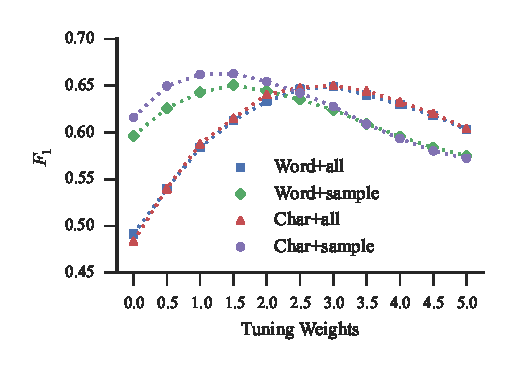
\includegraphics[width=.7\columnwidth]{figures/f1}
            \caption{\rmfamily{$F_1$ scores for varying values applied additively to the bias weights of the four annotation tags on the held-out 10k tuning subset.}}
            \label{figure:f1graph}
        \end{figure} 

        % \begin{figure}[htb]
        %     \centering
        %     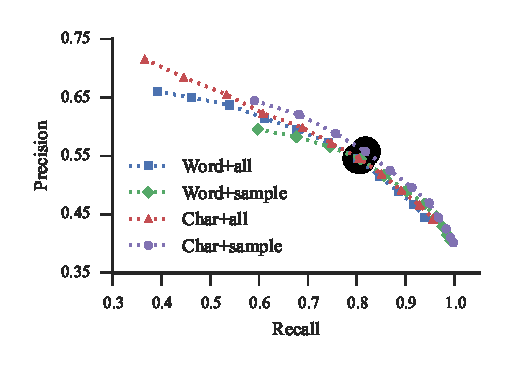
\includegraphics[width=.7\columnwidth]{figures/pr}
        %     \caption{\rmfamily{Precision vs. recall trade-off as the bias weights associated with the four annotation tags are varied on the held-out 10k tuning subset. The points yielding maximum $F_1$ scores are highlighted with black circles.}}
        %     \label{figure:prgraph}
        % \end{figure} 
    \end{block}
%%%%%%%%%%%%%%%%%%%
    \vskip2ex
%%%%%%%%%%%%%%%%%%%
    \begin{block}{Final Results}
        \begin{table}[ht!]
            \centering
            \small
            \begin{tabular}{lcccc}
            \toprule
            Model & Precision & Recall & $F_1$ \\
            \midrule
            \textsc{Random} & $0.3607$ & $0.6004$ & $0.4507$ \\
            \midrule
            \textsc{Knowlet} & $0.6241$ & $0.3685$ & $0.4634$ \\
            \textsc{NTNU-YZU} & $0.6717$ & $0.3805$ & $0.4858$ \\
            \textsc{HITS} & $0.3765$ & $0.948$ & $0.5389$ \\
            \textsc{UW-SU} & $0.4145$ & $0.8201$ & $0.5507$ \\
            \textsc{NTNU-YZU} & $0.5025$ & $0.7785$ & $0.6108$ \\
            \midrule
            \textsc{Char+sample} & $0.5112$ & $0.7841$ & \color{HarvardCrimson}{$0.6189$} \\
            \textsc{Combination} & $0.5444$ & $0.7413$ &  \color{HarvardCrimson}{$0.6278$} \\
            \bottomrule
            \end{tabular}
            \caption{\rmfamily{Our final system results on test (143,802 sentences evaluated on the Shared Task CodaLab server) are highlighted.}}
            \label{tab:test-results}
        \end{table}
    \end{block}
%%%%%%%%%%%%%%%%%%%
    \vskip1ex    
%%%%%%%%%%%%%%%%%%%
      \begin{block}{Conclusion}
       	\begin{itemize}
			\item Demonstrated comparatively strong results on the Shared Task, but many areas remain to be explored
			\item Future work to examine, among others:
			\vskip0.5ex
			\begin{itemize}
			    \item An end-to-end approach for languages such as Japanese
			    \item Approaches for incorporating additional error-free data
			    \item Performance on the correction task
			    \item User studies to assess the utility of correction vs. identification
			\end{itemize}
       	\end{itemize}
    \end{block}
%%%%%%%%%%%%%%%%%%%
    \end{column}
%%%%%%%%%%%%%%%%%%%%%%%%%%%%%%%%%%%%%% 
    \begin{column}{\sepwid}\end{column}			% empty spacer column
    \end{columns}
\end{frame}
\end{document}
